\lab{Fourier I: The Discrete Fourier Transform}{The Discrete Fourier Transform}
\objective{The analysis of periodic functions has many applications in pure and applied mathematics, especially in settings dealing with sound waves. The Fourier transform provides a way to analyze such periodic functions. In this lab, we implement the discrete Fourier transform and explore digital audio signals.}

% TODO:
%   - Note on Stereo vs. Mono.
%   - Note on scaling: scaling is only for wavfile format, so only scale
%       just before writing to file. Do not scale in other examples.
%       Show proper technique for scaling.
%   - Add implementation of FFT back in, right after naiive DFT (?)
%   - Recommended spec format: Jupyter Notebook.
%   - Possible additions: down sampling, etc.
%   - Explain that Fourier coefficients are complex. Absolute value!!!

\section*{Sound Waves} % ======================================================

Sounds are vibrations in the air around us.
The frequency and intensity of these vibrations determine how sound is perceived.
Sounds correspond physically to continuous functions, but they may be discretely approximated on a computer.
These discrete approximations can be made indistinguishable from a continuous signal.

\section*{Digital Audio Signals} % ============================================

There are two components of a digital audio signal: samples from the soundwave and a sample rate.
These correspond to amplitude and frequency, respectively.
A sample is a measurement of the amplitude of the wave at an instant in time.

\begin{comment} % TODO: This figure.
To see why the sample rate is necessary, consider an array with samples from a soundwave.
If we do not know how frequently those samples were collected then we can arbitrarily stretch or compress the soundwave to make a variety of sounds.
See Figure \ref{fig:comp_wave} for an illustration of this principle.

\begin{figure}
\centering
\caption{A picture of samples from a soundwave with varything frequencies.
It should be stretched or compressed to show how the frequency changes. Also describe how the sounds would be perceived.
The stretched out signal will sound deeper-ish.
Liiiiikkkkeeee tttthhhhhiiiiissss.
The shorter one will sound higher-ish.
Like this.}
\label{fig:comp_wave}
\end{figure}
\end{center}
\end{comment}

%However,
If we know at what rate the samples were taken, then we can construct the wave exactly as it was recorded.
In most applications, this sample rate will be measured in number of samples taken per second.
The standard rate for high quality audio is $44100$ equally spaced samples per second.

% Problem 1: Signal class.
\begin{problem}
Write a class called \li{Signal} for storing digital audio signals.
The constructor should accept a sample rate (an integer) and an array of samples (a NumPy array).
Store these inputs as attributes.

Write a method called \li{plot()} that generates the graph of the soundwave.
Use the sample rate to get the x-axis in terms of seconds.
See Figure \ref{fig:tada_sig} for an example.

%Finally, implement the \li{__add__()} magic method so that if two instances of \li{Signal} of the same length are added together, the sum of their signals are returned.% (as a new Signal object).
\end{problem}

\subsection*{Wave File Format} % ----------------------------------------------

One of the most common audio file formats across operating systems is the \emph{wave} format, also called \texttt{wav} after its file extension.
It is a lightweight, common standard that is in wide use.
SciPy has built-in tools to read and create \texttt{wav} files.
To read in a \texttt{wav} file, we can use the \li{read()} function that returns the file's sample rate and samples.
See Figure \ref{fig:tada_sig}.

\begin{lstlisting}
# Read from the sound file.
>>> from scipy.io import wavfile
>>> rate, wave = wavfile.read('tada.wav')

# To visualize the data, use the Signal class's plot function.
>>> sig = Signal(rate, wave)
>>> sig.plot()
\end{lstlisting}

\begin{figure}[ht]
\centering
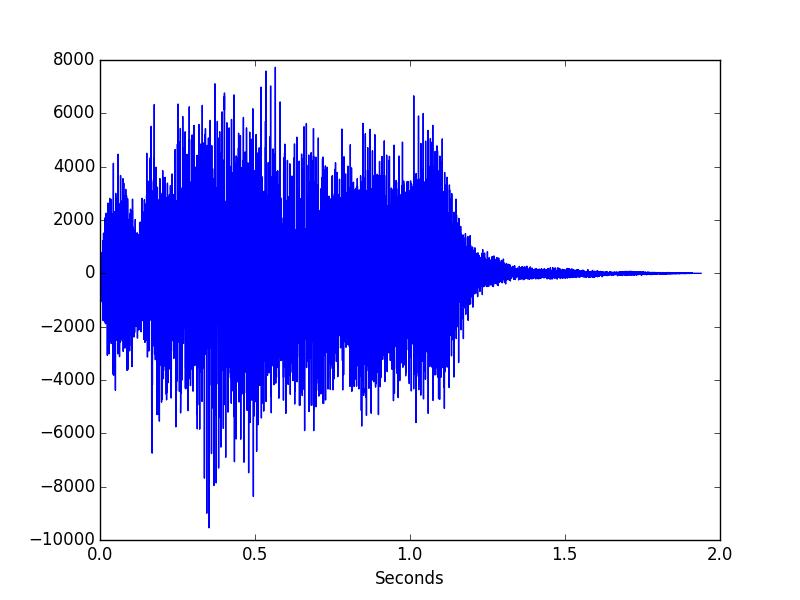
\includegraphics[width=\textwidth]{figures/tada.png}
\caption{The soundwave of \texttt{tada.wav}.}
\label{fig:tada_sig}
\end{figure}

Writing a signal to a file is also simple.
We use \li{wavfile.write()}, specifing the name of the new file, the sample rate, and the array of samples.

\begin{lstlisting}
# Write a random signal sampled at a rate of 44100 hz to my_sound.wav.
>>> wave = sp.random.randint(-32767, 32767, 30000)
>>> samplerate = 44100
>>> wavfile.write('my_sound.wav', samplerate, wave)
\end{lstlisting}

\subsection*{Scaling} % -------------------------------------------------------

The \li{wavfile.write()} function expects an array of 16 bit integers for the samples (whole numbers between $-32767$ and $32767$).
Therefore, waves may need to be scaled and converted to integers before being written to a file.

\begin{lstlisting}
# Generate random samples between -0.5 and 0.5.
>>> samples = sp.random.random(30000)-.5
# Scale the wave so that the samples are between -32767 and 32767.
>>> samples *= 32767*2
# Cast the samples as 16 bit integers.
>>> samples = sp.int16(samples)
\end{lstlisting}

The scaling technique in the above example works, but only because we knew beforehand that the values were in the interval $[-\frac{1}{2}, \frac{1}{2}]$.
If the entries of a wave are not scaled properly, the operating system may not know how to play the file.

% Problem 2: Signal.export
\begin{problem}
Add a method to the \li{Signal} class called \li{export()} that accepts a file name and generates a \texttt{.wav} file from the sample rate and the array of samples.
Scale the array of samples appropriately before writing to the outfile.
Ensure that your scaling technique is valid for arbitrary arrays of samples.
\end{problem}
% TODO: how do you determine if an array doesn't need to be scaled?

\section*{Creating Sounds in Python} % ========================================

In order to generate a sound in python, we need to sample the corresponding sine wave and then save it as an audio file.
For example, suppose that we want to generate a sound with a frequency of 500 hertz for 10 seconds.

\begin{lstlisting}
>>> samplerate = 44100
>>> frequency = 500
>>> length = 10         # Length in seconds of the desired sound.
\end{lstlisting}

Recall the the function $\sin(x)$ has a period of $2\pi$.
To create sounds, however, we want the period of our wave to be $1$, corresponding to $1$ second.
Thus, we will sample from the function
\[
\sin(2\pi xf)
\]
where $f$ is our desired frequency.

\begin{lstlisting}
# The lambda keyword is a shortcut for creating a one-line function.
>>> wave_function = lambda x: sp.sin(2*sp.pi*x*frequency)
\end{lstlisting}

In the following code, we generate a signal using three steps: first, find the correct step size given the sample rate.
Next, generate the points at which we wish to sample the wave.
Finally, sample the wave by passing the sample points to \li{wave_function}.
Then we can use our \li{Signal} class to plot the soundwave or write it to a file.

\begin{lstlisting}
# Calculate the step size, the sample points, and the sample values.
>>> stepsize = 1./samplerate
>>> sample_points = sp.arange(0, length, stepsize)
>>> samples = wave_function(sample_points)

# Use the Signal class to write the sound to a file.
>>> sinewave = Signal(samplerate, samples)
>>> sinewave.export("sine.wav")
\end{lstlisting}

The \li{export()} method should take care of scaling and casting the entries as 16-bit integers.

\begin{comment}
In this case, the samples are numbers between 0 to 1, taken from \li{wave_function()}.
However, \li{wavfile.write()} requires integeres between $-32767$ and $32767$.
Thus, we scale our sample points before creating a \texttt{.wav} file that can be played by the computer.

\begin{lstlisting}
>>> scaled_samples = sp.int16(samples*32767)
\end{lstlisting}

The \li{scaled_samples} array can now be written to a file using \li{wavfile.write()}.
This file can be played using media software included with most operating systems.
\end{comment}

% Problem 3: make a sound.
\begin{problem}
The `A' note occurs at a frequency of 440 hertz.
Generate the sine wave that corresponds to an `A' note being played for 5 seconds.

Once you have successfully generated the `A' note, experiment with different frequencies to generate different notes.
The following table shows some frequencies that correspond to common notes.

\begin{center}
\begin{tabular}{|c|c|}
\hline
Note & Frequency \\
\hline
A & 440 \\
B & 493.88 \\
C & 523.25 \\
D & 587.33 \\
E & 659.25 \\
F & 698.46 \\
G & 783.99 \\
\hline
\end{tabular}
\end{center}

Implement a function outside of the \li{Signal} class that accepts a frequency and a duration and returns an instance of the \li{Signal} class corresponding to the desired soundwave.
Sample at a rate of 44100 samples per second to create these sounds.
\end{problem}

\section*{Discrete Fourier Transform} % =======================================

\subsection*{Some Technicalities} % -------------------------------------------

Under the right conditions, a continuous periodic function may be represented as a sum of sine waves:
\[
f(x) = \displaystyle{\sum_{k=-\infty}^{\infty}} c_k \sin{kx}
\]
where the constants $c_k$ are called the \emph{Fourier coefficients}.

Such a transform also exists for discrete periodic functions.
Whereas the frequencies present in the continuous case are multiples of a sine wave with a period of 1, the discrete case is somewhat different.
The Fourier coefficients in the discrete case represent the amplitudes of sine waves whose periods are multiples of a ``fundamental frequency.''
The fundamental frequency is a sine wave with a period length equal to the amount of time of the signal.

The $k^{th}$ coefficient of a signal $\{x_0, .., x_{N-1}\}$ is calculated with the following formula:
\begin{align}
c_k = \displaystyle{\sum_{n=0}^{N-1}} x_n e^{\frac{2\pi ikn}{N}}\label{eq:ck}
\end{align}
where $i$ is the square root of $-1$.
This process is done for each $k$ from $0$ to $N-1$.
Thus there are just as many Fourier coefficients as samples from the orginal signal.

\begin{problem} % Problem 4: Naive DFT
Write a function that accepts a NumPy array and computes the discrete Fourier transform of the array using Equation \ref{eq:ck}.
Return the array of calculated coefficients.

SciPy has several methods for calculating the DFT of an array.
Use \li{scipy.fft()} or \li{scipy.fftpack.fft()} to check your implementation.
The naive method is significantly slower than SciPy's implementation, so test your function only on small arrays.
Can you calculate each coefficient $c_k$ in just one line of code?
\end{problem}

\begin{comment}
% TODO: a section on the FFT (!!!!)

% Problem 4.5: FFT - implement by hand, time / compare with SciPy, use a SciPy in the Signal class.

\begin{problem}
Implement the FFT.
\end{problem}
\end{comment}

\section*{Plotting the DFT} % =================================================

\begin{center}
\begin{figure}
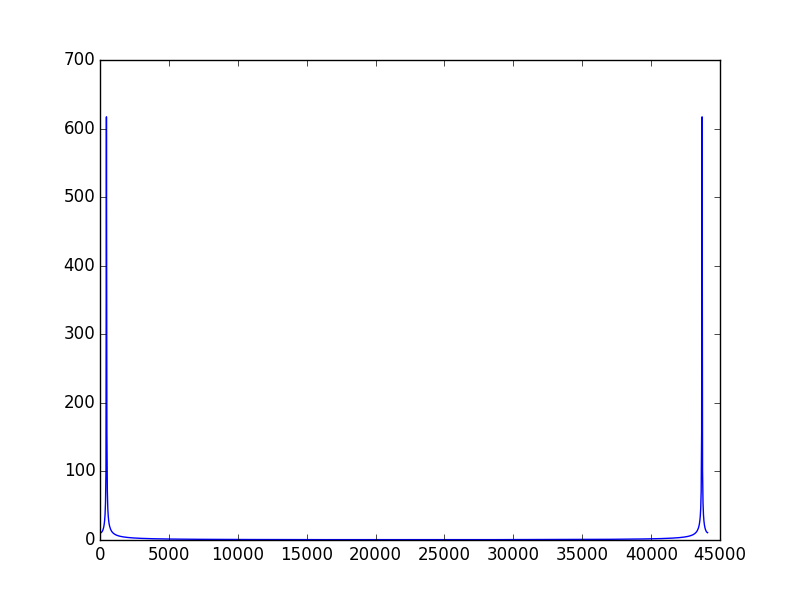
\includegraphics[scale=0.7]{figures/a_dft}
\caption{The magnitude of the coefficients of the discrete Fourier transform of an `A' note.  Notice that there are two spikes in the graph, the first around 440 on the x-axis.  This second spike is due to symmetries inherent in the DFT.  For our purposes we will mostly be concerned with the left side of the DFT plot.}
\label{fig:dft_a}
\end{figure}
\end{center}

The graph of the fourier transform of a sound file is useful in applications.
While the graph of the original signal gives information about the amplitude of a soundwave at certain points, the graph of the discrete Fourier transform  shows which frequencies are present in the signal.
Frequencies present in the signal have non-zero coefficients.
The magnitude of these coefficients corresponds to how influential the frequency is in the signal.
For example, the sounds that we generated in the previous section contained only one frequency.
If we created an `A' note at 440 hz, then the graph of the DFT would appear as in Figure \ref{fig:dft_a}.

On the other hand, the DFT of a more complicated soundwave will have many frequencies present.
Some of these frequencis correspond to the different tones present in the signal.
See Figure \ref{fig:dft_tada} for an example.

\begin{center}
\begin{figure}
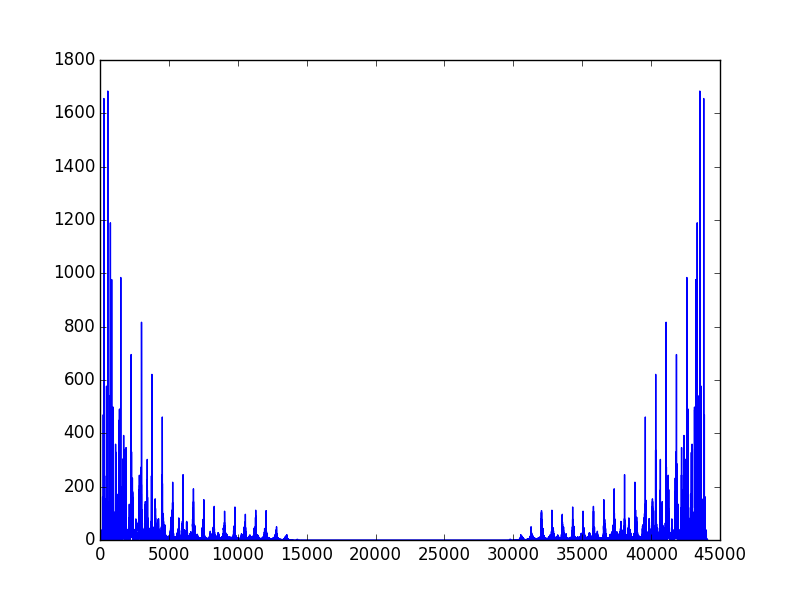
\includegraphics[scale=0.7]{figures/tada_dft}
\caption{The discrete Fourier transform of \texttt{tada.wav}.  Each spike in the graph corresponds to a frequency that is present in the signal.}
\label{fig:dft_tada}
\end{figure}
\end{center}

\subsection*{Fixing the x-axis} % ---------------------------------------------

If we take the DFT of a signal and then plot it without any other considerations, the x-axis will correspond to the index of the coefficients in the DFT and not their frequencies.
In a previous section, we mention that the ``fundamental frequency'' for the DFT corresponds to a sine wave whose period is the same as the length of the signal.
Thus, if unchanged, the x-axis gives us the number of times a particular sine wave cycles throughout the whole signal.
If we want to label the x-axis with the frequencies measured in hertz, or cycles per second, we will need to convert the units.
Fortunately, the bitrate is measured in samples per second.
Therfore, if we divide the frequency (given by the index) by the number of samples, and multiply by the sample rate, we end up with cycles per second, or hertz.

\begin{center}
    $\frac{\mbox{cycles}}{\mbox{samples}} \times \frac{\mbox{samples}}{\mbox{second}} = \frac{\mbox{cycles}}{\mbox{second}}$
\end{center}

\begin{lstlisting}
# Calculate the DFT and the x-values that correspond to the coefficients. Then
# convert the x-values so that they measure frequencies in hertz.
>>> dft = sp.fft(signal)
>>> x_vals = sp.arange(1,len(dft)+1, 1)*1. # Make them floats

# x_vals now corresponds to frequencies measured in cycles per signal length.
>>> x_vals = x_vals/len(signal)
>>> x_vals = x_vals*rate
\end{lstlisting}

\begin{comment} % Modify this problem so it's about calculating Hz.
\begin{problem}
Modify the \li{calculate_dft()} method so that in addition to calculating the Fourier coefficients, it also returns a list of their corresponding frequencies measured in hertz.
\end{problem}
\end{comment}

% Problem 5: plotting the DFT.
\begin{problem}
Update the \li{plot()} method in the \li{Signal} class so that it generates a single plot with two subplots: the original soundwave, and the magnitude of the coefficients of the DFT (as in Figure \ref{fig:dft_tada}).
Use one of SciPy's FFT implementations to calculate the DFT.
\end{problem}

% Problem 6: Generate a chord. TODO: be more specific on the requirements?
% Perhaps this problem should go earlier, or have more to do with the DFT.
\begin{problem}
A chord is a conjunction of several notes played together.
We can create a chord in Python by adding several sound waves together.
For example, to create a chord with `A', `C', and `E' notes, we generate the sound waves for each, as in the prior problem, and then add them together.

Create several chords and observe the plot of their DFT.
There should be as many spikes as there are notes in the plot.
Then create a sound that changes over time.

(Hints: you may consider implementing the \li{__add__()} magic method for the \li{Signal} class.
NumPy's \li{np.hstack()} and \li{np.vstack()} may also be helpful.)
\end{problem}

% Conclusion? Mono vs. Stereo?

% Additional ideas: write a method to reverse a sound?
